\chapter{Chapter Four}
\section{Discussion}
The number of cases with biased versus unbiased $Z_{DR}$ at CWKR was evenly split, with five each.
\subsection{Unbiased Cases}
The unbiased cases are given in Table \ref{unbiasedcases}
\begin{table}[h]
    \caption{Unbiased Cases}\label{unbiasedcases}
    \begin{center}
    \begin{tabular}{|l|c|c|c|}
    \hline
     Event & CWKR Median $Z_{DR}$ Bias & KBUF L3 $Z_{DR}$ Bias & Number of Matched Points\\
    \hline\hline
    2014-01-18 & -0.095 dB & -0.40 dB & 94,136 \\
    \hline
    2014-01-23 & -0.055 dB & -0.40 dB & 482,183 \\
    \hline
    2015-01-06 &  0.003 dB & -0.10 dB & 248,775 \\
    \hline
    2015-01-07 & -0.040 dB & -0.30 dB & 87,723 \\ 
    \hline
    2016-02-10 & -0.055 dB & 0.40 dB & 886,869 \\ 
    \hline
    \end{tabular}
    \end{center}
\end{table}
\begin{figure}[H]
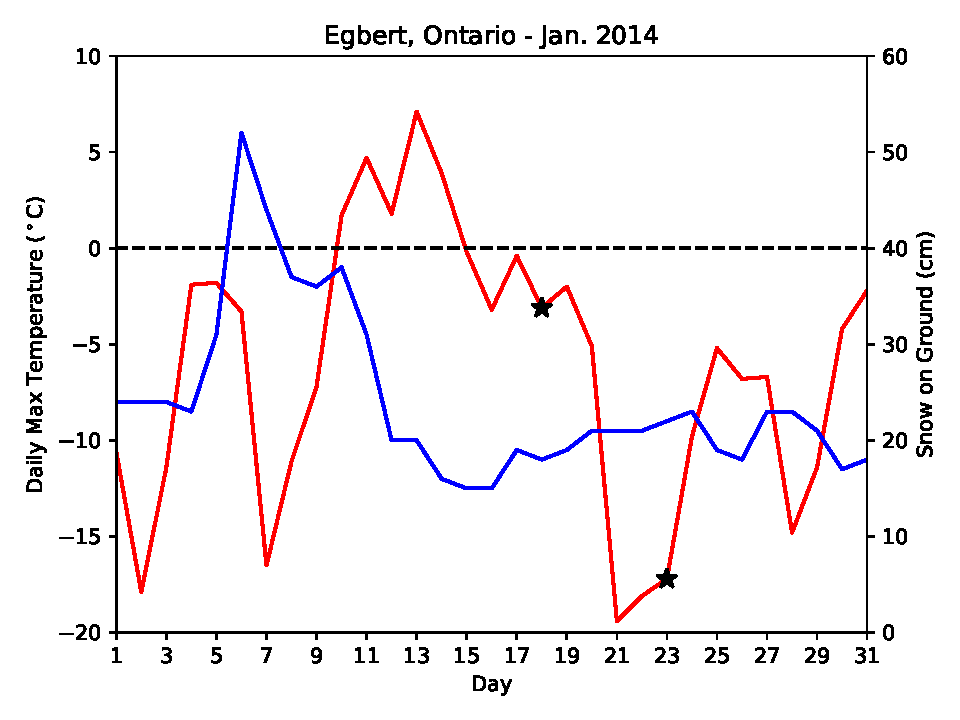
\includegraphics[width=\textwidth]{temp_egbert/Jan2014}
\caption{Daily Temperature and Snowfall data from the Egbert, ON Centre for Atmospheric Research Experiments (CARE) site, approximately 40 km north of CWKR. Case dates are indicated with a black star.} 
\label{fig:grid_ref_20140118}
\end{figure}
\subsection{Biased Cases}
\begin{table}[h]
    \caption{Biased Cases}\label{biasedcases}
    \begin{center}
    \begin{tabular}{|l|c|c|c|}
    \hline
     Event & CWKR Median $Z_{DR}$ Bias & KBUF L3 $Z_{DR}$ Bias & Number of Matched Points\\
    \hline\hline
    2014-02-01 & 0.217 dB & -0.20 dB & 310,631 \\
    \hline
    2015-02-06 & 0.283 dB & 0.00 dB & 143,563 \\
    \hline
    2015-02-14 & 0.377 dB & -0.10 dB & 331,154 \\
    \hline
    2015-02-18 & 0.296 dB & -0.10 dB & 177,124 \\
    \hline
    2016-12-15 & -0.465 dB & -0.28 dB & 53,383 \\
    \hline
    \end{tabular}
    \end{center}
\end{table}